\documentclass[12pt,a4paper,oneside]{report}

%-------------------- Page layout and fonts --------------------------
\usepackage[a4paper,left=1.25in,right=1in,top=1in,bottom=1in,headheight=15pt]{geometry}
% Font: LaTeX default Computer Modern (cmr) throughout --- do not load other font packages
\usepackage{eso-pic}             % page border on front-matter pages
\usepackage{setspace}
\onehalfspacing
\usepackage{microtype}

%-------------------- Packages ---------------------------------------
\usepackage{graphicx}
\usepackage{amsmath,amssymb}
\usepackage{booktabs,tabularx,multirow,longtable,array}
\usepackage{float}
\usepackage[font=small,labelfont=bf]{caption}
\usepackage{enumitem}
\usepackage[dvipsnames,table]{xcolor}
\usepackage{tikz}
\usetikzlibrary{arrows.meta,positioning,shapes.geometric,fit,backgrounds}
\usepackage{pgfplots}
\pgfplotsset{compat=1.17}
\usepackage{algorithm}
\usepackage{algpseudocode}
\usepackage{listings}
\usepackage[most]{tcolorbox}
\usepackage{fancyhdr}
\usepackage{titlesec}
\usepackage{hyperref}
\hypersetup{
    bookmarksopen=true,
    colorlinks=true,
    citecolor=blue,
    linkcolor=blue,
    urlcolor=blue
}

%=====================================================================
%  PROJECT DETAILS --- EDIT THIS BLOCK
%=====================================================================
\newcommand{\ProjectTitle}{SolarScreen: An Agentic Pre-Screener for Rooftop-Solar Net-Metering Interconnection Applications}
% Short title for the page header (shorten if it does not fit on one line)
\newcommand{\HeaderTitle}{SolarScreen: Agentic Net-Metering Interconnection Pre-Screener}
\newcommand{\TeamNo}{07}
\newcommand{\AcademicYear}{2026--27}
\newcommand{\SubmissionDate}{12 November 2026}
% Team members: USN and Name (delete the 4th row in the tables if you have only 3 members)
\newcommand{\USNa}{1BM23CD001}  \newcommand{\NameA}{Student Name One}
\newcommand{\USNb}{1BM23CD002}  \newcommand{\NameB}{Student Name Two}
\newcommand{\USNc}{1BM23CD003}  \newcommand{\NameC}{Student Name Three}
\newcommand{\USNd}{1BM23CD004}  \newcommand{\NameD}{Student Name Four}
% Course lead
\newcommand{\GuideName}{Dr. Kalyan Nagaraj}
\newcommand{\GuideDesig}{Assistant Professor}

%=====================================================================
%  GUIDANCE SWITCH: set to \guidancefalse before final submission
%=====================================================================
\newif\ifguidance
\guidancetrue

%-------------------- Colours and boxes -------------------------------
\definecolor{bmsblue}{RGB}{0,51,102}
\definecolor{guidebg}{RGB}{232,240,252}
\definecolor{dobg}{RGB}{230,245,233}
\definecolor{dontbg}{RGB}{252,232,232}
\definecolor{samplecol}{RGB}{40,55,80}

% "What to write here" box
\newcommand{\guide}[1]{%
  \ifguidance
  \begin{tcolorbox}[enhanced,breakable,colback=guidebg,colframe=bmsblue,
    boxrule=0.6pt,arc=2pt,left=6pt,right=6pt,top=4pt,bottom=4pt,
    fonttitle=\bfseries\small,title={What to write here},
    before upper={\small\setstretch{1.1}}]
  #1
  \end{tcolorbox}
  \fi}

% Do / Don't box (two columns)
\newcommand{\dodont}[2]{%
  \ifguidance
  \begin{tcolorbox}[enhanced,breakable,sidebyside,sidebyside align=top seam,
    colback=dobg,colbacklower=dontbg,colframe=gray!60,boxrule=0.5pt,arc=2pt,
    lefthand ratio=0.5,left=5pt,right=5pt,top=4pt,bottom=4pt,
    fontupper=\small\setstretch{1.05},fontlower=\small\setstretch{1.05}]
  \textbf{\textcolor{ForestGreen}{\checkmark\ Do}}
  \begin{itemize}[leftmargin=12pt,itemsep=1pt,topsep=2pt]#1\end{itemize}
  \tcblower
  \textbf{\textcolor{BrickRed}{$\times$ Don't}}
  \begin{itemize}[leftmargin=12pt,itemsep=1pt,topsep=2pt]#2\end{itemize}
  \end{tcolorbox}
  \fi}

% Page budget note for each chapter
\newcommand{\pagebudget}[1]{%
  \ifguidance\noindent{\small\textcolor{bmsblue}{\textbf{Expected length:} #1 pages}}\par\medskip\fi}

% Sample content marker (sample text is shown in dark slate colour)
\newenvironment{sample}
  {\par\noindent{\footnotesize\bfseries\textcolor{BrickRed}{[SAMPLE --- replace with your own content]}}\par\color{samplecol}}
  {\par\medskip}

%-------------------- Headers and footers ----------------------------
% Main body (Chapter 1 onwards): project title right in header, CSE (Data Science) left and
% page number right in footer, with double rules. Front matter: page border, page number only.
% Double rules (thick + thin, 1.5pt apart), drawn with \hrule so no line spacing is inserted
\newcommand{\DoubleHeadRule}{\vskip 2pt{\color{bmsblue}%
  \hrule width\headwidth height 1.2pt\vskip 1.5pt\hrule width\headwidth height 0.4pt}\vskip -5.1pt}
\newcommand{\DoubleFootRule}{\vskip-\footruleskip\vskip-3.1pt{\color{bmsblue}%
  \hrule width\headwidth height 0.4pt\vskip 1.5pt\hrule width\headwidth height 1.2pt}\vskip\footruleskip}
\fancypagestyle{mainbody}{%
  \fancyhf{}%
  \fancyhead[R]{\small\itshape\HeaderTitle}%
  \fancyfoot[L]{\small CSE (Data Science)}%
  \fancyfoot[R]{\small\thepage}%
  \renewcommand{\headrulewidth}{1pt}\renewcommand{\footrulewidth}{1pt}%
  \renewcommand{\headrule}{\DoubleHeadRule}\renewcommand{\footrule}{\DoubleFootRule}}
\fancypagestyle{frontmatter}{%
  \fancyhf{}\fancyfoot[C]{\small\thepage}%
  \renewcommand{\headrulewidth}{0pt}\renewcommand{\footrulewidth}{0pt}%
  \renewcommand{\headrule}{}\renewcommand{\footrule}{}}
% Double page border (front matter only)
\newcommand{\PageBorder}{%
  \AddToShipoutPictureBG{\AtPageLowerLeft{%
    \setlength{\unitlength}{1pt}%
    \begin{tikzpicture}[remember picture,overlay]
      \draw[bmsblue,line width=1.6pt] ([xshift=1.2cm,yshift=1.2cm]current page.south west)
        rectangle ([xshift=-1.2cm,yshift=-1.2cm]current page.north east);
      \draw[bmsblue,line width=0.5pt] ([xshift=1.35cm,yshift=1.35cm]current page.south west)
        rectangle ([xshift=-1.35cm,yshift=-1.35cm]current page.north east);
    \end{tikzpicture}}}}

%-------------------- Chapter heading style --------------------------
\titleformat{\chapter}[display]
  {\normalfont\bfseries\centering}
  {\Large\textcolor{bmsblue}{CHAPTER \thechapter}}{6pt}{\LARGE\MakeUppercase}
\titlespacing*{\chapter}{0pt}{-10pt}{24pt}
\titleformat{\section}{\normalfont\large\bfseries}{\thesection}{0.6em}{}
\titleformat{\subsection}{\normalfont\normalsize\bfseries}{\thesubsection}{0.6em}{}

%-------------------- Code listing style -----------------------------
\lstset{basicstyle=\ttfamily\footnotesize,breaklines=true,frame=single,
  backgroundcolor=\color{gray!6},numbers=left,numberstyle=\tiny\color{gray},
  keywordstyle=\color{bmsblue}\bfseries,commentstyle=\color{ForestGreen},
  stringstyle=\color{BrickRed},showstringspaces=false,columns=fullflexible,keepspaces=true}

\begin{document}

%=====================================================================
%  INSTRUCTIONS PAGE (shown only while \guidancetrue)
%=====================================================================
\ifguidance
\pagenumbering{gobble}
\thispagestyle{empty}
\begin{center}
{\Large\bfseries\textcolor{bmsblue}{Instructions to Students --- Read Before You Start}}\\[4pt]
{\small (This page disappears when you set \texttt{\textbackslash guidancefalse})}
\end{center}

\begin{tcolorbox}[colback=guidebg,colframe=bmsblue,arc=2pt,boxrule=0.6pt]
\small\setstretch{1.15}
\textbf{1. Length.} The main body (Chapter~1 to Chapter~10) must be \textbf{between 30 and 50 pages}.
Front matter (title page to list of abbreviations), references and appendices are \emph{not} counted.
Reports below 30 pages or above 50 pages will lose marks under ``Report quality''.

\medskip
\textbf{2. Tone.} Write in a clear, formal, \textbf{academic} style. Use complete sentences and
the third person or ``we''. Do not use slang, chat language, emojis, exclamation marks or
marketing language (``revolutionary'', ``game-changing'', ``cutting-edge'').

\medskip
\textbf{3. Honesty.} Report only what your system actually does. Every number in the report
must come from your own runs. The numbers in the SAMPLE blocks are \textbf{illustrative only}
and must never appear in your report. Honest negative results are acceptable; fabricated results
are an academic-integrity violation.

\medskip
\textbf{4. Citations.} Cite every external idea, dataset, model, framework, figure and piece of code
in IEEE style, e.g.\ ``ReAct~\cite{yao2023react} interleaves reasoning and acting.''
Do not copy text from papers, websites or AI tools without attribution.

\medskip
\textbf{5. Figures and tables.} Every figure and table must have a number, a caption, and
must be referred to in the text before it appears (``as shown in Fig.~4.1''). Figures must be
legible when printed; do not paste low-resolution screenshots of code. \textbf{The architecture
diagram (Chapter~4) must be drawn in LaTeX using TikZ or an equivalent LaTeX package}, not inserted
as an image.

\medskip
\textbf{6. Formatting.} Do not change the font (Computer Modern), font size (12\,pt), line
spacing (1.5), margins, page borders, header/footer or heading styles of this template.

\medskip
\textbf{7. The running example.} The SAMPLE blocks use one fictional project,
\emph{SolarScreen}, to show the expected depth and style. It is an illustration only.
Your report must describe your own project.

\medskip
\textbf{8. Before submission.} Set \texttt{\textbackslash guidancefalse}, recompile twice,
and check that no SAMPLE text, red markers or placeholder names remain. Submit the PDF,
the slides (PDF), and the repository link by \textbf{\SubmissionDate}.
\end{tcolorbox}

\begin{tcolorbox}[colback=white,colframe=gray!60,arc=2pt,boxrule=0.5pt,title=\textbf{Suggested page budget},colbacktitle=gray!20,coltitle=black]
\small
\begin{tabularx}{\linewidth}{@{}l X r@{}}
\toprule
\textbf{Ch.} & \textbf{Chapter} & \textbf{Pages} \\ \midrule
1 & Introduction & 4--6 \\
2 & Literature Survey and Existing Practice & 4--6 \\
3 & Requirements and System Analysis & 3--4 \\
4 & Agent Design and Architecture & 5--7 \\
5 & Agentic Concepts Demonstrated & 3--4 \\
6 & Implementation & 5--7 \\
7 & Observability and Evaluation & 4--6 \\
8 & Experimentation & 2--4 \\
9 & Limitations, Ethics and Safety & 2--3 \\
10 & Conclusion and Future Work & 1--2 \\ \midrule
 & \textbf{Total (main body)} & \textbf{33--49} \\ \bottomrule
\end{tabularx}
\end{tcolorbox}
\clearpage
\fi

%=====================================================================
%  TITLE PAGE
%=====================================================================
\pagenumbering{gobble}
\PageBorder
\pagestyle{frontmatter}
\begin{titlepage}
\centering
\setstretch{1.2}
{\large\bfseries B.M.S. COLLEGE OF ENGINEERING}\\[2pt]
{\normalsize (Autonomous Institute, Affiliated to VTU, Belagavi)}\\[2pt]
{\normalsize Bull Temple Road, Basavanagudi, Bengaluru -- 560019}\\[12pt]

\includegraphics[width=3.2cm]{logo.png}\\[14pt]
{\normalsize A Mini-Project Report on}\\[10pt]
{\Large\bfseries\textcolor{bmsblue}{\ProjectTitle}}\\[14pt]
{\normalsize Submitted as the Alternative Assessment Tool (AAT) for the course}\\[2pt]
{\normalsize\bfseries Agentic AI (26CD7PEAAI)}\\[2pt]
{\normalsize of}\\[2pt]
{\normalsize\bfseries Bachelor of Engineering}\\[2pt]
{\normalsize in}\\[2pt]
{\normalsize\bfseries Computer Science and Engineering (Data Science)}\\[14pt]
{\normalsize Submitted by (Team No.\ \TeamNo)}\\[6pt]
\renewcommand{\arraystretch}{1.3}
\begin{tabular}{l@{\hspace{1.5cm}}l}
\textbf{\USNa} & \textbf{\NameA} \\
\textbf{\USNb} & \textbf{\NameB} \\
\textbf{\USNc} & \textbf{\NameC} \\
\textbf{\USNd} & \textbf{\NameD} \\
\end{tabular}\\[16pt]
{\normalsize Course Lead}\\[4pt]
{\large\bfseries \GuideName}\\[2pt]
{\normalsize \GuideDesig, Department of CSE (Data Science)}\\[2pt]
{\normalsize B.M.S. College of Engineering, Bengaluru}\\[16pt]
\vfill
{\normalsize\bfseries Department of Computer Science and Engineering (Data Science)}\\[2pt]
{\normalsize B.M.S. College of Engineering, Bengaluru}\\[2pt]
{\normalsize Academic Year \AcademicYear}
\end{titlepage}

%=====================================================================
%  FRONT MATTER
%=====================================================================
\pagenumbering{roman}
\setcounter{page}{2}

%-------------------- Certificate ------------------------------------
\chapter*{Certificate}
\addcontentsline{toc}{chapter}{Certificate}
\thispagestyle{frontmatter}
\begin{center}

\includegraphics[width=2.2cm]{logo.png}\\[6pt]
{\bfseries B.M.S. College of Engineering, Bengaluru}\\
Department of Computer Science and Engineering (Data Science)
\end{center}
\vspace{10pt}
This is to certify that the mini-project entitled \textbf{``\ProjectTitle''} has been carried out by
\NameA\ (\USNa), \NameB\ (\USNb), \NameC\ (\USNc) and \NameD\ (\USNd), bona fide students of
B.M.S. College of Engineering, Bengaluru, as the Alternative Assessment Tool (AAT) for the evaluation
of the course \textbf{Agentic AI (26CD7PEAAI)}, Semester VII, Bachelor of Engineering in Computer
Science and Engineering (Data Science), during the academic year \AcademicYear. The work has been
evaluated through the four project reviews prescribed for the course, and this report satisfies the
requirements of the AAT component of the said course.

\vspace{70pt}
\noindent\hfill
\begin{minipage}[t]{0.62\textwidth}\raggedleft
\rule{6cm}{0.4pt}\\
\textbf{\GuideName}\\
Course Lead, Agentic AI (26CD7PEAAI)\\
\GuideDesig, Dept. of CSE (Data Science)\\
B.M.S. College of Engineering, Bengaluru\\[10pt]
Date: \rule{3.5cm}{0.4pt}
\end{minipage}

%-------------------- Abstract ---------------------------------------
\chapter*{Abstract}
\addcontentsline{toc}{chapter}{Abstract}
\thispagestyle{frontmatter}
\guide{A single paragraph of 200--300 words, followed by 4--6 keywords. Answer, in order:
(1) Which sector and what decision? (2) Why is it niche and why does it need an agent rather than
a single LLM call? (3) What did you build (agent type, patterns, tools)? (4) How did you evaluate
it? (5) What is the headline result, with a number? (6) What is the main limitation?}
\dodont{\item Write it last, after all results are final.
\item Include at least one quantitative result.
\item Make it understandable without reading the report.}
{\item Do not cite references, figures or tables.
\item Do not use abbreviations without expanding them.
\item Do not exceed one paragraph or 300 words.}
\begin{sample}
Rooftop-solar applicants in India are frequently rejected or delayed because their net-metering
interconnection applications are incomplete or violate distribution-company (DISCOM) feeder-capacity
limits, and the relevant rules are spread across lengthy standard operating procedures. This report
presents \emph{SolarScreen}, an agentic pre-screening assistant that checks an application against
the applicable procedures and feeder data before it is submitted. The agent follows a
plan-and-execute loop with reflection; it uses agentic retrieval-augmented generation over a corpus of
42 DISCOM procedure documents, a feeder-capacity lookup tool, and a structured-output validator, and
it pauses for human confirmation before issuing a ``reject'' recommendation. Every run is traced,
and quality is measured on a hand-labelled set of 60 applications using rule-based checks and an
LLM-as-a-judge rubric. On this set, SolarScreen identified missing documents with an F1-score of
0.88 and produced correctly cited verdicts in 85\% of cases, compared with 61\% for a single-prompt
baseline. An A/B experiment showed that adding a retrieval-grading step improved citation accuracy by
14 percentage points at the cost of 1.9 additional seconds per application. The system is advisory
only and is limited by the coverage of the procedure corpus, which currently includes two DISCOMs.

\medskip
\noindent\textbf{Keywords:} agentic AI, retrieval-augmented generation, plan-and-execute,
net metering, rooftop solar, human-in-the-loop.
\end{sample}

%-------------------- Lists ------------------------------------------
\tableofcontents
\listoffigures
\addcontentsline{toc}{chapter}{List of Figures}
\listoftables
\addcontentsline{toc}{chapter}{List of Tables}

\chapter*{List of Abbreviations}
\addcontentsline{toc}{chapter}{List of Abbreviations}
\thispagestyle{frontmatter}
\guide{List every abbreviation used in the report in alphabetical order. Expand each abbreviation
again at its first use in the main text.}
\begin{sample}
\begin{tabular}{@{}p{2.8cm}l@{}}
API & Application Programming Interface \\
DISCOM & Distribution Company \\
HITL & Human-in-the-Loop \\
LLM & Large Language Model \\
RAG & Retrieval-Augmented Generation \\
ReAct & Reasoning and Acting \\
SOP & Standard Operating Procedure \\
\end{tabular}
\end{sample}

%=====================================================================
%  MAIN BODY
%=====================================================================
\clearpage
\ClearShipoutPictureBG
\pagestyle{mainbody}
\fancypagestyle{plain}{\pagestyle{mainbody}}
\pagenumbering{arabic}

%---------------------------------------------------------------------
\chapter{Introduction}
%---------------------------------------------------------------------
\pagebudget{4--6}
\guide{This chapter introduces the sector, the problem and the decision your agent supports, and
explains why an agentic approach is justified. A reader who stops after this chapter should know
exactly what you built and why.}

\section{Background}
\guide{Describe the sector and the real-world process in which your problem occurs. Give one or two
facts with citations that show the problem matters (volume, cost, delay, risk). Two to three
paragraphs.}
\dodont{\item Start from the real-world setting, not from LLMs.
\item Support every factual claim with a citation.}
{\item Do not open with ``In today's fast-paced world'' or ``AI is changing everything''.
\item Do not write a general history of artificial intelligence.}
\begin{sample}
Under the net-metering regulations notified by state electricity regulatory commissions, a consumer
who installs a rooftop photovoltaic system may export surplus energy to the grid and offset it
against consumption. Before the system can be connected, the consumer or installer must submit an
interconnection application to the distribution company (DISCOM), which checks the application
against technical limits such as the sanctioned load and the hosting capacity of the distribution
transformer and feeder~\cite{example-sop}.

Each DISCOM publishes its own standard operating procedure (SOP), and these documents differ in
document requirements, capacity thresholds and timelines. Installers handling applications across
several DISCOMs must therefore consult long and frequently revised procedure documents, which leads
to incomplete submissions and avoidable rejections.
\end{sample}

\section{Problem Statement}
\guide{State the problem in one precise paragraph, ending with a single sentence in bold that names
the decision the agent supports. The problem must be specific enough that a reader can tell whether
your system solves it.}
\dodont{\item Name the user, the input, the output and the decision.
\item Keep it to one paragraph.}
{\item Do not state a vague goal (``to use AI to improve solar adoption'').
\item Do not describe your solution here.}
\begin{sample}
An installer preparing a net-metering application has no reliable way to know, before submission,
whether the application is complete and whether the proposed capacity is acceptable on the
consumer's feeder. The relevant rules are distributed across procedure documents, circulars and
feeder-capacity tables that must be read together.
\textbf{The decision supported is: should this application be submitted as it is, corrected first,
or referred to the DISCOM for a capacity study?}
\end{sample}

\section{Motivation and Why Agentic AI}
\guide{Explain why a plain script, a rule engine, or a single LLM prompt is insufficient, and which
agentic capabilities (tool use, retrieval, planning, reflection, human-in-the-loop) the problem
genuinely requires. This section is assessed directly in the viva.}
\dodont{\item Compare explicitly with simpler alternatives.
\item Link each agentic capability to a concrete property of the problem.}
{\item Do not claim an agent is needed merely because it is ``more intelligent''.
\item Do not list agentic features that your system does not use.}
\begin{sample}
A rule engine could check a fixed list of documents, but the rules differ between DISCOMs and change
through circulars, so encoding them by hand is costly and brittle. A single LLM prompt cannot
reliably consult feeder-capacity data, nor can it verify that its answer is grounded in the current
procedure. The task is naturally multi-step: identify the DISCOM, retrieve the applicable clauses,
query the feeder capacity, compare, and decide. It therefore requires (i) controlled retrieval over
procedures, (ii) a tool call to the capacity data, (iii) an explicit plan, and (iv) human confirmation
before an adverse recommendation, which together motivate an agentic design.
\end{sample}

\section{Objectives}
\guide{List three to six objectives. Each must be specific and measurable, and each must be
answered somewhere in Chapters 7--8.}
\dodont{\item Begin each objective with a verb (design, implement, evaluate).
\item Make at least one objective quantitative.}
{\item Do not write objectives you did not attempt.
\item Do not mix objectives with features.}
\begin{sample}
\begin{enumerate}[itemsep=2pt]
\item To design a plan-and-execute agent that pre-screens net-metering applications against DISCOM
procedures and feeder-capacity data.
\item To implement agentic retrieval with relevance grading and re-querying over the procedure corpus.
\item To instrument every run with step-level traces and a human-approval step for adverse verdicts.
\item To evaluate verdict accuracy and citation correctness on a labelled set of 60 applications.
\item To compare, through an A/B experiment, retrieval with and without a grading step.
\end{enumerate}
\end{sample}

\section{Scope of the Project}
\guide{State what is included and, equally important, what is excluded. Clear exclusions protect you
in the viva.}
\dodont{\item List inclusions and exclusions separately.
\item Keep the scope small enough to finish.
}
{\item Do not promise features you will not build.
\item Do not leave the scope implicit.
}
\begin{sample}
The system covers residential rooftop installations up to 10\,kW in two DISCOMs. It does not submit
applications, does not handle commercial or industrial consumers, and produces advisory output only;
the final decision rests with the installer and the DISCOM.
\end{sample}

\section{Organisation of the Report}
\guide{One short paragraph listing what each subsequent chapter contains.}
\dodont{\item Mention every chapter once.
}
{\item Do not repeat the chapter titles as a bulleted list.
}

\begin{sample}
Chapter~2 reviews existing practice and related work. Chapter~3 states the requirements.
Chapter~4 presents the architecture, and Chapter~5 maps it to the agentic concepts of the course.
Chapter~6 describes the implementation, Chapter~7 the observability and evaluation, and Chapter~8
the experiment. Chapter~9 discusses limitations, ethics and safety, and Chapter~10 concludes.
\end{sample}

%---------------------------------------------------------------------
\chapter{Literature Survey and Existing Practice}
%---------------------------------------------------------------------
\pagebudget{4--6}
\guide{Show that you understand (a) how the problem is handled today in the sector and (b) the
technical literature on the agentic techniques you use. End with a clear statement of the gap your
project addresses. Review at least 10 sources, of which at least 6 should be peer-reviewed papers.}

\section{Existing Practice in the Sector}
\guide{Describe the current manual or software process: who does it, which tools are used, and where
it fails. Use sources such as regulator documents, industry reports or interviews you conducted.}
\dodont{\item Describe the real workflow step by step.
\item Cite official or primary sources.}
{\item Do not rely only on blog posts or marketing pages.
\item Do not invent statistics.}
\begin{sample}
At present, installers check applications manually against the DISCOM checklist. Some DISCOMs
provide online portals that validate file formats but not the content of the documents or the
feeder-capacity limits~\cite{example-sop}. Capacity problems are therefore discovered only after
submission, typically during the DISCOM's technical feasibility study.
\end{sample}

\section{Related Technical Work}
\guide{Organise the literature by theme, not paper by paper. Typical themes for this course are
tool-using language models, retrieval-augmented generation, planning and reflection, multi-agent
systems, and evaluation of LLM output. For each theme, summarise the key idea and how it relates to
your project.}
\dodont{\item Group papers by theme and compare them.
\item Say how each work relates to your design.
\item Paraphrase in your own words and cite.
}
{\item Do not write one paragraph per paper with no comparison.
\item Do not copy abstracts.
\item Do not cite papers you have not read.
}

\subsection{Reasoning and Acting with Tools}
\begin{sample}
Yao et al.~\cite{yao2023react} proposed ReAct, in which a language model interleaves reasoning traces
with actions such as search queries, allowing it to gather information before answering. Schick et
al.~\cite{schick2023toolformer} showed that language models can learn when and how to call external
tools. SolarScreen adopts tool calling for the feeder-capacity lookup but uses an explicit plan rather
than free-form interleaving, so that each step can be traced and bounded.
\end{sample}

\subsection{Retrieval-Augmented Generation}
\begin{sample}
Lewis et al.~\cite{lewis2020rag} introduced retrieval-augmented generation (RAG), which conditions
generation on retrieved passages. Later work made retrieval adaptive: Self-RAG~\cite{asai2024selfrag}
learns to decide when to retrieve and to critique its own output, and Corrective RAG~\cite{yan2024crag}
grades retrieved documents and falls back to alternative retrieval when they are weak. SolarScreen
follows the corrective pattern with a lightweight relevance grader.
\end{sample}

\subsection{Reflection and Multi-Agent Collaboration}
\begin{sample}
Reflexion~\cite{shinn2023reflexion} improves agents through verbal self-feedback across attempts.
AutoGen~\cite{wu2023autogen} provides a framework in which several specialised agents converse to
complete a task. A survey by Wang et al.~\cite{wang2024survey} categorises such systems by profile,
memory, planning and action modules.
\end{sample}

\subsection{Evaluation of LLM-Based Systems}
\begin{sample}
Zheng et al.~\cite{zheng2023judge} studied the use of strong language models as judges and reported
high agreement with human preferences, while noting position and verbosity biases. SolarScreen
therefore combines an LLM judge with deterministic rule-based checks.
\end{sample}

\section{Comparative Summary}
\guide{Summarise the most relevant works in a table with consistent columns. The last row should be
your project, so that the gap is visible.}
\dodont{\item Use the same columns for every row.
\item Cite each row.
}
{\item Do not include more than 8--10 rows.
\item Do not tick features a work does not have.
}

\begin{sample}
\begin{table}[H]
\centering
\caption{Comparison of related approaches with the proposed system}
\label{tab:litcompare}
\small
\begin{tabularx}{\linewidth}{@{}p{3.6cm} X c c c@{}}
\toprule
\textbf{Work} & \textbf{Key idea} & \textbf{Tools} & \textbf{Adapt.\ RAG} & \textbf{HITL} \\
\midrule
ReAct~\cite{yao2023react} & Interleaved reasoning and acting & \checkmark & -- & -- \\
RAG~\cite{lewis2020rag} & Retrieval-conditioned generation & -- & -- & -- \\
CRAG~\cite{yan2024crag} & Retrieval grading and fallback & -- & \checkmark & -- \\
Manual DISCOM checklist & Human review against SOP & -- & -- & \checkmark \\
\textbf{SolarScreen (ours)} & Plan-and-execute pre-screening & \checkmark & \checkmark & \checkmark \\
\bottomrule
\end{tabularx}
\end{table}
\end{sample}

\section{Research Gap}
\guide{Two or three sentences that follow directly from the table: what is missing, and how your
project addresses it.}
\dodont{\item Derive the gap from the works you reviewed.}
{\item Do not claim that ``no work exists'' unless you have searched thoroughly.}
\begin{sample}
Existing practice relies on manual checks, and general agent frameworks have not been applied to
interconnection pre-screening. No reviewed system combines grounded retrieval over DISCOM procedures,
feeder-capacity verification and human confirmation in a single traceable workflow; this project
addresses that gap.
\end{sample}

%---------------------------------------------------------------------
\chapter{Requirements and System Analysis}
%---------------------------------------------------------------------
\pagebudget{3--4}
\guide{Translate the problem into concrete requirements that the design in Chapter~4 must satisfy
and the evaluation in Chapter~7 must test.}

\section{Stakeholders and Users}
\guide{Identify who uses the system, who is affected by its output, and what each needs from it.}
\dodont{\item Name real roles in the sector.
}
{\item Do not write ``all users'' or ``everyone''.
}

\begin{sample}
The primary users are rooftop-solar installers. Secondary stakeholders are consumers, who benefit from
fewer rejections, and DISCOM engineers, who receive more complete applications.
\end{sample}

\section{Functional Requirements}
\guide{Number every requirement (FR1, FR2, \ldots) so that you can refer to it later.}
\dodont{\item Write each requirement as a testable statement.}
{\item Do not write requirements that you did not implement.}
\begin{sample}
\begin{description}[itemsep=1pt,font=\normalfont\bfseries]
\item[FR1] The system shall accept an application as a structured form and attached PDF documents.
\item[FR2] The system shall identify the DISCOM and retrieve the applicable procedure clauses.
\item[FR3] The system shall query feeder capacity for the given transformer code.
\item[FR4] The system shall output a verdict (\emph{submit}, \emph{correct first}, \emph{refer}) with cited clauses.
\item[FR5] The system shall request human approval before issuing a \emph{refer} verdict.
\end{description}
\end{sample}

\section{Non-Functional Requirements}
\guide{Quantified constraints on latency, cost, reliability, traceability and safety.}
\dodont{\item Give a number for each requirement.
\item Make cost and loop bounds explicit.
}
{\item Do not write ``the system should be fast and user-friendly''.
}
\begin{sample}
\begin{description}[itemsep=1pt,font=\normalfont\bfseries]
\item[NFR1] Latency: a verdict within 30 seconds for 95\% of applications.
\item[NFR2] Cost: at most 15 LLM calls per application (bounded loops).
\item[NFR3] Traceability: every run stored as a step-level trace.
\item[NFR4] Safety: no verdict without at least one cited clause; abstain otherwise.
\end{description}
\end{sample}

\section{Data Sources}
\guide{For each data source give its origin, size, format, licence, and how you obtained or
created it. If any data is synthetic or mocked, say so explicitly.}
\dodont{\item State size, format and licence for each source.
\item Mark synthetic or mocked data clearly.
}
{\item Do not use data whose licence forbids it.
\item Do not hide that data is synthetic.
}
\begin{sample}
\begin{table}[H]
\centering
\caption{Data sources used in SolarScreen}
\label{tab:data}
\small
\begin{tabularx}{\linewidth}{@{}l X l l@{}}
\toprule
\textbf{Source} & \textbf{Description} & \textbf{Size} & \textbf{Origin} \\ \midrule
Procedure corpus & DISCOM SOPs and circulars (PDF) & 42 docs & Public websites \\
Feeder capacity & Transformer-wise hosting capacity & 1{,}200 rows & Mocked (synthetic) \\
Test applications & Labelled sample applications & 60 & Created by team \\
\bottomrule
\end{tabularx}
\end{table}
\end{sample}

\section{Hardware and Software Requirements}
\guide{List the hardware and software actually used, with versions.}
\dodont{\item Give exact versions in the appendix.
}
{\item Do not list generic requirements such as ``a computer with internet''.
}
\begin{sample}
Development used laptops with 16\,GB RAM and Python~3.11. The agent uses LangGraph for
orchestration, a hosted LLM through an API, Chroma as the vector store, and LangSmith for tracing.
Exact versions are listed in Appendix~\ref{app:run}.
\end{sample}

\section{Feasibility}
\guide{Briefly discuss technical feasibility, cost (API usage), and time, and how you limited the scope
to finish within the semester.}
\dodont{\item Estimate API cost per run and in total.
}
{\item Do not ignore cost or rate limits.
}

\begin{sample}
The average run uses 9 LLM calls and about 6{,}000 tokens. With the selected model, the full evaluation
of 60 applications in three repetitions costs approximately [amount], which is within the team's
budget. External DISCOM portals were not accessed; feeder data were mocked to avoid dependency on
unavailable APIs.
\end{sample}


%---------------------------------------------------------------------
\chapter{Agent Design and Architecture}
%---------------------------------------------------------------------
\pagebudget{5--7}
\guide{This is the central design chapter. Present the architecture diagram, describe every
component, state the agentic patterns you selected, show the data and control flow, and justify each
design decision against alternatives.}

\section{System Architecture}
\guide{Include one clear architecture diagram drawn by you. \textbf{The architecture diagram must be
drawn in LaTeX using TikZ} (or an equivalent LaTeX drawing package such as PGF or \texttt{tikz-uml});
the sample in Figure~\ref{fig:arch} is TikZ code you can adapt. Screenshots or images exported from
draw.io, PowerPoint or other tools are not accepted for this figure. Every box in the diagram must be
explained in Section~4.2.}
\dodont{\item Draw the diagram in TikZ so it is sharp and editable.
\item Use consistent shapes: agents, tools, data stores, humans.
\item Label every arrow with what flows along it.}
{\item Do not insert the architecture as a PNG/JPG screenshot.
\item Do not paste a framework's generic diagram.
\item Do not include components that do not exist in your code.}
\begin{sample}
Figure~\ref{fig:arch} shows the architecture of SolarScreen. A planner decomposes the screening task
into steps, an executor carries out each step using tools, a reflector checks the draft verdict, and a
human approval gate is invoked for adverse outcomes.

\begin{figure}[H]
\centering
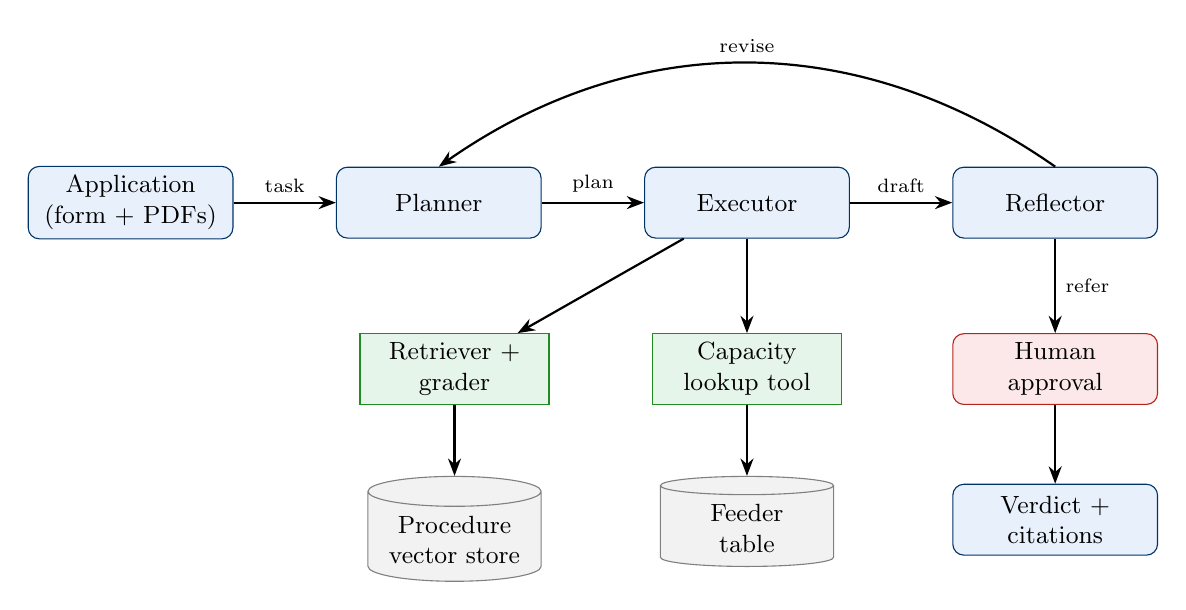
\begin{tikzpicture}[
  node distance=0.9cm and 1.3cm,
  agent/.style={draw=bmsblue,fill=guidebg,rounded corners,minimum width=2.6cm,minimum height=0.9cm,align=center,font=\small},
  tool/.style={draw=ForestGreen,fill=dobg,minimum width=2.4cm,minimum height=0.8cm,align=center,font=\small},
  store/.style={draw=gray,fill=gray!10,cylinder,shape border rotate=90,aspect=0.2,minimum width=2.2cm,minimum height=1.0cm,align=center,font=\small},
  human/.style={draw=BrickRed,fill=dontbg,rounded corners,minimum width=2.6cm,minimum height=0.8cm,align=center,font=\small},
  arr/.style={-{Stealth[length=2.2mm]},thick}]
\node[agent] (in) {Application\\(form + PDFs)};
\node[agent, right=of in] (plan) {Planner};
\node[agent, right=of plan] (exec) {Executor};
\node[tool, below=1.2cm of exec] (cap) {Capacity\\lookup tool};
\node[tool, left=of cap] (ret) {Retriever +\\grader};
\node[store, below=0.9cm of ret] (vs) {Procedure\\vector store};
\node[store, below=0.9cm of cap] (db) {Feeder\\table};
\node[agent, right=of exec] (refl) {Reflector};
\node[human, below=1.2cm of refl] (hitl) {Human\\approval};
\node[agent, below=1.0cm of hitl] (out) {Verdict +\\citations};
\draw[arr] (in) -- node[above,font=\scriptsize]{task} (plan);
\draw[arr] (plan) -- node[above,font=\scriptsize]{plan} (exec);
\draw[arr] (exec) -- (ret);
\draw[arr] (exec) -- (cap);
\draw[arr] (ret) -- (vs);
\draw[arr] (cap) -- (db);
\draw[arr] (exec) -- node[above,font=\scriptsize]{draft} (refl);
\draw[arr] (refl.north) to[bend right=35] node[above,font=\scriptsize]{revise} (plan.north);
\draw[arr] (refl) -- node[right,font=\scriptsize]{refer} (hitl);
\draw[arr] (hitl) -- (out);
\end{tikzpicture}
\caption{Architecture of SolarScreen (sample)}
\label{fig:arch}
\end{figure}
\end{sample}

\section{Component Description}
\guide{One subsection per component: its responsibility, its inputs and outputs, the model or
algorithm it uses, and its failure behaviour.}
\dodont{\item Describe every box in the architecture diagram.
\item State what happens when the component fails.
}
{\item Do not paste code here; code belongs in Chapter~6.
\item Do not describe components that are not in the diagram.
}

\subsection{Planner}
\begin{sample}
The planner receives the application and produces an ordered list of at most six steps in JSON. It
is prompted with the list of available tools and a schema; plans that fail schema validation are
regenerated once and otherwise rejected.
\end{sample}
\subsection{Executor and Tools}
\begin{sample}
The executor runs each step, calling the retriever or the capacity tool as required, and records the
observation. Tool errors are caught and returned to the executor as observations rather than raised.
\end{sample}
\subsection{Retriever and Relevance Grader}
\begin{sample}
The retriever returns the top five chunks by cosine similarity. A grader scores each chunk as relevant
or irrelevant; if fewer than two are relevant, the query is rewritten and retrieval is repeated once.
\end{sample}
\subsection{Reflector and Human Approval Gate}
\begin{sample}
The reflector checks that every claim in the draft verdict is supported by a cited clause. Verdicts of
type \emph{refer} are paused for installer approval before release.
\end{sample}

\section{Selected Agentic Patterns and Justification}
\guide{Name each pattern (ReAct, plan-and-execute, reflection, corrective RAG, supervisor multi-agent,
etc.), explain why you chose it, and state which alternative you rejected and why.}
\dodont{\item Present a short table: pattern, where used, why chosen, alternative rejected.}
{\item Do not list patterns only because they are popular.}
\begin{sample}
\begin{table}[H]
\centering
\caption{Agentic patterns and design justification}
\label{tab:patterns}
\small
\begin{tabularx}{\linewidth}{@{}l l >{\raggedright\arraybackslash}X l@{}}
\toprule
\textbf{Pattern} & \textbf{Where} & \textbf{Reason} & \textbf{Alternative rejected} \\ \midrule
Plan-and-execute & Planner/executor & Steps are known in advance; easy to bound and trace & Free-form ReAct \\
Corrective RAG & Retriever & Procedures are long; weak retrieval must be detected & Single-shot RAG \\
Reflection & Reflector & Every claim must be cited & No self-check \\
HITL gate & Before \emph{refer} & Adverse outcome affects the consumer & Fully automatic \\
\bottomrule
\end{tabularx}
\end{table}
\end{sample}

\section{Control Flow and Agent State}
\guide{Describe how control moves between components (a state machine or graph is ideal) and what is
stored in the shared state. Show how and where loops terminate.}
\dodont{\item Name every termination condition.
\item List the fields of the shared state.
}
{\item Do not leave any loop without an upper bound.
}
\begin{sample}
The workflow is implemented as a directed graph whose shared state holds the application, the plan,
the observations, the draft verdict, a step counter and a retry counter. The graph terminates when the
reflector accepts the verdict, when the step counter reaches six, or when the retry counter reaches two;
in the last two cases the agent abstains and explains why.
\end{sample}

\section{Data Flow}
\guide{Trace one input end-to-end through the system, naming the data at each stage. A sequence
diagram is recommended.}
\dodont{\item Follow one concrete example input.
}
{\item Do not describe data flow only in abstract terms.
}

\begin{sample}
An application for a 5\,kW system in transformer zone T-114 enters as a JSON form with four PDFs.
The planner emits a five-step plan. Step~2 retrieves seven clauses from the procedure store;
step~3 returns a hosting capacity of 38\,kW with 31\,kW already allocated. The executor compares the
remaining 7\,kW with the requested 5\,kW, the reflector confirms that both claims are cited, and the
verdict \emph{submit} is returned with three clause citations.
\end{sample}


%---------------------------------------------------------------------
\chapter{Agentic Concepts Demonstrated}
%---------------------------------------------------------------------
\pagebudget{3--4}
\guide{Map your system explicitly to the concept checklist in Section~5 of the project guidelines.
All five Mandatory concepts must be covered. For each concept, give concrete evidence: a trace
excerpt, a screenshot, a log line or a figure number.}

\section{Concept Coverage Matrix}
\begin{sample}
\begin{table}[H]
\centering
\caption{Coverage of the agentic-concept checklist}
\label{tab:concepts}
\small
\begin{tabularx}{\linewidth}{@{}l l c X@{}}
\toprule
\textbf{Tier} & \textbf{Concept} & \textbf{Status} & \textbf{Evidence} \\ \midrule
Mandatory & Tool / function use & \checkmark & Capacity lookup, Fig.~5.1 \\
Mandatory & Agentic RAG & \checkmark & Grader and re-query, Listing~5.1 \\
Mandatory & Planning and reasoning & \checkmark & Plan in trace, Fig.~5.1 \\
Mandatory & Observability / tracing & \checkmark & Section~7.1 \\
Mandatory & Evaluation & \checkmark & Chapter~7 \\
Bonus & Multi-agent collaboration & -- & Not implemented \\
Bonus & Memory & Partial & Short-term state only \\
Bonus & Human-in-the-loop and guardrails & \checkmark & Section~4.2.4 \\
Bonus & Durable workflow & -- & Not implemented \\
Bonus & Experimentation & \checkmark & Chapter~8 \\
\bottomrule
\end{tabularx}
\end{table}
\end{sample}
\dodont{\item Mark concepts you did not implement honestly as ``Not implemented''.
\item Point to a specific figure, listing or trace for each tick.}
{\item Do not tick a concept without evidence.
\item Do not count a framework feature you never used.}

\section{Evidence for Each Concept}
\guide{One subsection per ticked concept. Show a short trace excerpt or screenshot and explain in two or
three sentences what it demonstrates.}
\dodont{\item Use real traces from your own runs.
\item Crop and annotate screenshots so the key step is readable.}
{\item Do not stage or edit traces.
\item Do not show evidence for a concept that is not in the matrix.}

\subsection{Tool Use}
\begin{sample}
In the trace shown in Fig.~5.1 (insert your screenshot), the executor calls the
capacity-lookup tool (\texttt{feeder\_capacity}) with transformer ID T-114, receives the remaining capacity, and uses it in the
next reasoning step to compare against the requested capacity.
\end{sample}

\subsection{Agentic RAG}
\begin{sample}
Listing~\ref{lst:regrade} shows a run in which the grader rejected four of the five retrieved chunks.
The agent rewrote the query to include the DISCOM name and retrieved three relevant chunks on the
second attempt.

\begin{lstlisting}[language=Python,caption={Trace excerpt showing retrieval grading and re-query (sample)},label={lst:regrade}]
{"step": 2, "node": "retrieve", "query": "document checklist net metering",
 "graded": {"relevant": 1, "irrelevant": 4}, "action": "rewrite_query"}
{"step": 3, "node": "retrieve", "query": "BESCOM net metering document checklist 2025",
 "graded": {"relevant": 3, "irrelevant": 2}, "action": "proceed"}
\end{lstlisting}
\end{sample}
\subsection{Planning and Reasoning}
\begin{sample}
The planner produced the five-step plan shown in the trace; after the reflector rejected a draft with
an uncited claim, the plan was revised to add a retrieval step for the missing clause.
\end{sample}

\subsection{Observability}
\begin{sample}
All 180 evaluation runs are stored as traces with per-step inputs, outputs, latency and token counts
(Section~7.1).
\end{sample}

\subsection{Evaluation}
\begin{sample}
Quality is measured with rule-based metrics and an LLM-judge rubric on a labelled set of 60
applications (Chapter~7).
\end{sample}

\subsection{Bonus Concepts}
\begin{sample}
A human-approval gate pauses every \emph{refer} verdict (Fig.~5.2, insert screenshot); the A/B
experiment in Chapter~8 provides the experimentation bonus. Multi-agent collaboration and durable
workflows were not implemented.
\end{sample}


%---------------------------------------------------------------------
\chapter{Implementation}
%---------------------------------------------------------------------
\pagebudget{5--7}
\guide{Describe how the design was built: the technology stack, the data pipeline, the core algorithm,
the prompts, the tools, how loops are bounded, and the repository structure. Another student should be
able to reproduce your system from this chapter and Appendix~\ref{app:run}.}

\section{Technology Stack}
\begin{sample}
\begin{table}[H]
\centering
\caption{Technology stack}
\label{tab:stack}
\small
\begin{tabular}{@{}ll@{}}
\toprule
\textbf{Layer} & \textbf{Choice (version)} \\ \midrule
Language & Python 3.11 \\
Orchestration & LangGraph 0.x \\
LLM & [Provider and model name] \\
Embeddings and vector store & [Embedding model], Chroma \\
Tracing & LangSmith \\
Interface & Streamlit \\
\bottomrule
\end{tabular}
\end{table}
\end{sample}
\dodont{\item Give exact versions and model names.
\item Explain why each major choice was made.}
{\item Do not list libraries you installed but did not use.}

\section{Data Preparation and Indexing}
\guide{Explain how raw data was cleaned, chunked, embedded and stored. State chunk size, overlap and
the embedding model, and justify these choices.}
\dodont{\item Give the exact parameters used.
\item Justify the chunk size.
}
{\item Do not say ``the data was preprocessed'' without detail.
}

\begin{sample}
The 42 PDFs were converted to text, headers and footers were removed, and the text was split into
chunks of 800 characters with 100-character overlap so that most clauses remain within one chunk. Each
chunk carries the DISCOM name, document title and clause number as metadata, which are used for
citations. The corpus produced 3{,}410 chunks.
\end{sample}


\section{Core Agent Loop}
\guide{Present the main loop as pseudocode (not raw code). Show where the loop is bounded.}
\dodont{\item Use the algorithm environment.
\item Explain the pseudocode line by line in text.
}
{\item Do not paste long blocks of source code.
}

\begin{sample}
\begin{algorithm}[H]
\caption{SolarScreen agent loop (sample)}
\label{alg:loop}
\begin{algorithmic}[1]
\Require application $a$, max steps $S=6$, max retries $R=2$
\State $P \gets \textsc{Plan}(a)$; \quad $s \gets 0$; \quad $r \gets 0$
\While{$s < S$}
  \State $o \gets \textsc{Execute}(P[s])$ \Comment{tool call or retrieval}
  \State append $o$ to observations; $s \gets s+1$
\EndWhile
\State $v \gets \textsc{Draft}(a,\text{observations})$
\While{\textbf{not} \textsc{Reflect}$(v)$ \textbf{and} $r < R$}
  \State $v \gets \textsc{Revise}(v)$; $r \gets r+1$
\EndWhile
\If{$r = R$} \State \Return \textsc{Abstain}(``insufficient evidence'') \EndIf
\If{$v.\text{type} = \textit{refer}$} \State \textsc{AwaitHumanApproval}$(v)$ \EndIf
\State \Return $v$
\end{algorithmic}
\end{algorithm}
\end{sample}

\section{Tools and Function Definitions}
\guide{For each tool give its name, purpose, input schema, output schema and error handling. Mocked
tools must be identified as mocked.}
\dodont{\item Present tools in a table.
\item Describe the error behaviour.
}
{\item Do not hide that a tool is mocked.
}

\begin{sample}
\begin{table}[H]
\centering
\caption{Tools available to the agent}
\small
\begin{tabularx}{\linewidth}{@{}l X X@{}}
\toprule
\textbf{Tool} & \textbf{Input / output} & \textbf{Notes} \\ \midrule
\texttt{feeder\_capacity} & transformer ID $\rightarrow$ capacity, allocated (kW) & Mocked table; returns error for unknown ID \\
\texttt{retrieve\_clauses} & query, DISCOM $\rightarrow$ top-5 chunks with metadata & Chroma vector store \\
\texttt{validate\_docs} & document list $\rightarrow$ missing items & Rule-based check \\
\bottomrule
\end{tabularx}
\end{table}
\end{sample}


\section{Prompt Design}
\guide{Show the system prompt of each agent (shortened if long) in a listing or in Appendix~D, and
explain the key instructions, such as the output schema, citation rules and abstention rules.}
\dodont{\item Explain why each instruction is there.
\item Mention prompt revisions that changed behaviour.
}
{\item Do not include API keys or personal data in prompts shown.
}

\begin{sample}
\begin{lstlisting}[language={},numbers=none,caption={Reflector system prompt (shortened, sample)}]
You are a compliance reviewer. For each claim in the draft verdict, check that
it is supported by a cited clause in the provided context. If any claim is
unsupported, return {"accept": false, "unsupported": [...]}. Never invent
clause numbers. If evidence is insufficient, recommend abstention.
\end{lstlisting}
\end{sample}


\section{Guardrails and Loop Bounds}
\guide{List every guardrail: maximum steps, maximum retries, timeout, input validation, output schema
validation, and refusal or abstention rules.}
\dodont{\item Give the numeric value of every bound.
}
{\item Do not allow any unbounded loop on a paid API.
}

\begin{sample}
The agent stops after 6 executor steps or 2 reflection retries, and each LLM call has a 20-second
timeout. Inputs are validated against a JSON schema; outputs that fail schema validation are rejected.
The agent abstains when no clause with similarity above 0.55 is retrieved.
\end{sample}


\section{User Interface}
\guide{One or two screenshots of the interface with a short description. Keep this brief; the interface
is not the focus of the course.}
\dodont{\item Show the screen where the agent's reasoning is visible.
}
{\item Do not spend more than one page on the interface.
}

\begin{sample}
Fig.~6.1 (insert screenshot) shows the Streamlit interface: the left panel accepts the application,
and the right panel shows the plan, each step's observation, and the final verdict with citations.
\end{sample}


\section{Repository Structure}
\guide{Show the folder layout and describe the purpose of each main file.}
\dodont{\item Keep the repository clean and documented.
}
{\item Do not commit API keys, virtual environments or large data files.
}
\begin{sample}
\begin{lstlisting}[language={},numbers=none,caption={Repository layout (sample)}]
solarscreen/
|-- README.md          # setup and run instructions
|-- requirements.txt
|-- data/              # corpus, feeder table (mocked), test set
|-- src/
|   |-- graph.py       # LangGraph workflow
|   |-- tools.py       # capacity lookup, validator
|   |-- retrieval.py   # indexing, retriever, grader
|   |-- prompts/       # system prompts
|-- eval/              # golden set, metrics, judge rubric
|-- app.py             # Streamlit interface
\end{lstlisting}
\end{sample}

%---------------------------------------------------------------------
\chapter{Observability and Evaluation}
%---------------------------------------------------------------------
\pagebudget{4--6}
\guide{Show that you can see inside the agent (tracing) and that you measured how well it works
(evaluation). Every number in this chapter must come from your own runs.}

\section{Tracing and Monitoring}
\guide{Describe what is captured per run (steps, inputs, outputs, latency, tokens, cost) and include one
annotated trace screenshot.}
\dodont{\item Annotate the screenshot to point out the agentic behaviour.}
{\item Do not include an unreadable full-page screenshot.}
\begin{sample}
Each run is recorded in LangSmith as a tree of spans, one per graph node, with inputs, outputs, latency
and token usage. Fig.~7.1 (insert annotated screenshot) highlights a run in which the grader triggered
a re-query and the reflector requested one revision. Mean latency per run was [x]\,s and mean token
usage [y].
\end{sample}


\section{Evaluation Dataset}
\guide{Describe how the test set was built, its size, how labels were assigned and by whom, and its
class distribution. A small, carefully labelled set is better than a large, unlabelled one.}
\dodont{\item Report the class distribution.
\item Keep the test set separate from development data.}
{\item Do not tune prompts on the test set.}
\begin{sample}
The evaluation set contains 60 applications created by the team from public templates: 25 complete,
20 with missing documents and 15 exceeding feeder capacity. Two team members labelled each application
independently; disagreements (4 cases) were resolved by discussion.
\end{sample}

\section{Metrics and Evaluation Rubric}
\guide{Define every metric precisely, with a formula where appropriate. If you use an LLM as a judge,
give the rubric and report agreement with human labels on a subset.}
\dodont{\item Define each metric before reporting it.
\item Validate the LLM judge against human labels.
}
{\item Do not rely only on ``the output looked good''.
}

\begin{sample}
Missing-document detection is measured by precision $P$, recall $R$ and
$F_1 = \dfrac{2PR}{P+R}$. Verdict accuracy is the fraction of applications whose verdict matches the
label. Citation correctness is judged by an LLM judge using a three-point rubric (correct, partially
correct, incorrect), which agreed with a human annotator on 18 of 20 sampled cases.
\end{sample}

\section{Baselines}
\guide{Compare against at least one simpler baseline, for example a single prompt with no tools or RAG
without grading.}
\dodont{\item Use the same model and data for baseline and system.
}
{\item Do not use a deliberately weak baseline.
}

\begin{sample}
Two baselines were used: (i) a single prompt containing the application and the full checklist,
with no tools; and (ii) the full pipeline with retrieval grading disabled. Both used the same model and
temperature as SolarScreen.
\end{sample}


\section{Results}
\guide{Present results in tables and figures, then interpret them in text. Discuss failures as well
as successes.}
\dodont{\item Report means with spread (standard deviation or range) where runs vary.
\item Explain why the system fails on its failure cases.}
{\item \textbf{Never copy the illustrative numbers in this template.}
\item Do not report only the best run.}
\begin{sample}
\begin{table}[H]
\centering
\caption{Evaluation results on the 60-application test set \textcolor{BrickRed}{(ILLUSTRATIVE --- replace)}}
\label{tab:results}
\small
\begin{tabular}{@{}lccc@{}}
\toprule
\textbf{System} & \textbf{Missing-doc F1} & \textbf{Verdict acc.} & \textbf{Citation correct} \\ \midrule
Single-prompt baseline & 0.62 & 0.58 & 61\% \\
RAG without grading & 0.79 & 0.72 & 71\% \\
\textbf{SolarScreen (full)} & \textbf{0.88} & \textbf{0.83} & \textbf{85\%} \\
\bottomrule
\end{tabular}
\end{table}
As Table~\ref{tab:results} shows, the full system outperforms both baselines on all three metrics.
Most remaining errors (6 of 10) occurred on applications citing circulars newer than the corpus.
\end{sample}

\section{Error Analysis}
\guide{Group the failures into categories, give counts and one example per category, and state what
would fix each category.}
\dodont{\item Show at least one real failure example.
}
{\item Do not omit failures to make results look better.
}

\begin{sample}
Of the 10 incorrect verdicts, 6 involved circulars newer than the corpus (fix: periodic corpus
update), 3 were caused by misread scanned documents (fix: better OCR), and 1 was a wrong
transformer ID supplied by the user (fix: input validation against the feeder list).
\end{sample}


%---------------------------------------------------------------------
\chapter{Experimentation}
%---------------------------------------------------------------------
\pagebudget{2--4}
\guide{Describe one controlled experiment comparing two variants (A/B, or offline versus online), and
the design decision it informed.}

\section{Hypothesis}
\guide{State one testable hypothesis about two variants of your system.}
\dodont{\item Make the hypothesis falsifiable.
}
{\item Do not compare variants that differ in many ways at once.
}
\begin{sample}
Adding a relevance-grading step to retrieval (variant B) will increase citation correctness compared
with plain top-$k$ retrieval (variant A), at an acceptable latency cost.
\end{sample}

\section{Experimental Setup}
\guide{State what was varied, what was held fixed (model, temperature, data), the number of runs, and
the metrics.}
\dodont{\item Change only one factor between variants.
\item Repeat runs to account for randomness.
}
{\item Do not change the test set between variants.
}

\begin{sample}
Variant A uses plain top-5 retrieval; variant B adds the relevance grader and one re-query. The model,
temperature (0.2), prompts and the 60-application test set were held fixed. Each variant was run three
times; we report the mean citation correctness and mean latency.
\end{sample}


\section{Results}
\guide{Present the comparison as a table or chart, with spread across runs.}
\dodont{\item Report both the benefit and the cost.
}
{\item Do not hide a latency or cost increase.
}
\begin{sample}
\begin{figure}[H]
\centering
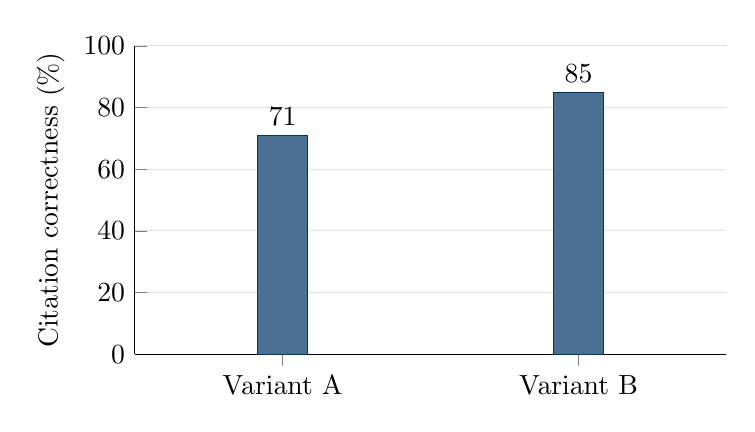
\begin{tikzpicture}
\begin{axis}[ybar,bar width=18pt,width=0.75\linewidth,height=5.5cm,
  ymin=0,ymax=100,ylabel={Citation correctness (\%)},
  symbolic x coords={Variant A,Variant B},xtick=data,
  nodes near coords,nodes near coords align={vertical},
  enlarge x limits=0.5,axis lines*=left,ymajorgrids,grid style={gray!25}]
\addplot[fill=bmsblue!70,draw=bmsblue] coordinates {(Variant A,71) (Variant B,85)};
\end{axis}
\end{tikzpicture}
\caption{Citation correctness for the two retrieval variants \textcolor{BrickRed}{(ILLUSTRATIVE --- replace)}}
\label{fig:ab}
\end{figure}
\end{sample}

\section{Discussion and Decision}
\guide{State whether the hypothesis was supported, discuss the trade-off, and state the decision you
took as a result.}
\dodont{\item State the decision explicitly (``we adopted variant B because\ldots'').}
{\item Do not declare a winner from a single run.}
\begin{sample}
Variant B improved citation correctness by 14 percentage points (mean of three runs) while increasing
mean latency by 1.9\,s per application, which remains within NFR1. The hypothesis was supported, and
variant B was adopted as the default configuration.
\end{sample}


%---------------------------------------------------------------------
\chapter{Limitations, Ethics and Safety}
%---------------------------------------------------------------------
\pagebudget{2--3}
\guide{Be honest and specific. Reviewers give credit for clear thinking about failure modes, not for
claiming that the system has none.}

\section{Limitations}
\guide{List the main limitations of data, method and evaluation.}
\dodont{\item Be specific and honest.
}
{\item Do not write ``the system has no major limitations''.
}
\begin{sample}
The corpus covers only two DISCOMs, the feeder data are synthetic, and the test set is small and
team-constructed, so the reported results may not generalise.
\end{sample}

\section{Failure Modes and Guardrails}
\guide{List the ways the agent can fail (hallucinated clause, wrong tool input, loop exhaustion, prompt
injection in documents) and the guardrail that addresses each.}
\dodont{\item Pair each failure mode with its mitigation.
}
{\item Do not list risks without mitigations.
}

\begin{sample}
\begin{table}[H]
\centering
\caption{Failure modes and mitigations}
\small
\begin{tabularx}{\linewidth}{@{}>{\raggedright\arraybackslash}X >{\raggedright\arraybackslash}X@{}}
\toprule
\textbf{Failure mode} & \textbf{Mitigation} \\ \midrule
Fabricated clause number & Reflector rejects uncited claims; citations checked against metadata \\
Weak retrieval & Grader with one re-query, then abstention \\
Loop exhaustion & Step and retry limits with explicit abstention message \\
Instructions hidden in uploaded PDFs & Document text treated as data; tool calls restricted to an allow-list \\
\bottomrule
\end{tabularx}
\end{table}
\end{sample}


\section{Ethical and Responsible-Use Considerations}
\guide{Discuss who could be harmed by a wrong output, privacy of user data, bias, and why the system
remains advisory and human-confirmed (Section~8.3 of the guidelines).}
\dodont{\item State clearly that the output is advisory.}
{\item Do not present the agent's output as a legal, medical or financial decision.}
\begin{sample}
An incorrect \emph{submit} verdict could cause a consumer's application to be rejected and delayed.
The system therefore labels every verdict as advisory, shows its citations, and requires human
approval for adverse verdicts. Uploaded applications may contain personal data; they are processed
locally and are not stored after the session.
\end{sample}


%---------------------------------------------------------------------
\chapter{Conclusion and Future Work}
%---------------------------------------------------------------------
\pagebudget{1--2}
\section{Conclusion}
\guide{Restate the problem, what was built, and the main quantitative results. Revisit each objective
from Section~1.4 and state whether it was met.}
\dodont{\item Answer each objective explicitly.}
{\item Do not introduce new results here.
\item Do not overstate the impact.}
\begin{sample}
This report presented SolarScreen, an agentic pre-screener for net-metering applications. All five
objectives were met: the plan-and-execute agent with corrective retrieval achieved a missing-document
F1-score of 0.88 and 85\% citation correctness on the test set, and the A/B experiment justified the
retrieval-grading step.
\end{sample}

\section{Future Work}
\guide{Three to five concrete, feasible extensions that follow from your limitations.}
\dodont{\item Link each item to a stated limitation.
}
{\item Do not list vague ideas such as ``use better AI''.
}

\begin{sample}
\begin{enumerate}[itemsep=1pt]
\item Extend the corpus to all DISCOMs in the state, with automatic detection of new circulars.
\item Replace the mocked feeder table with official hosting-capacity data where available.
\item Add persistent memory of past applications to detect recurring errors by installers.
\end{enumerate}
\end{sample}


%=====================================================================
%  REFERENCES
%=====================================================================
\guide{Use IEEE style. Cite at least 10 sources. Every reference must be cited in the text, and every
citation must appear here. Prefer papers, official documents and documentation over blogs. The entries
below are real works you may cite if you use them; delete those you do not cite.}
\begin{thebibliography}{99}
\addcontentsline{toc}{chapter}{References}
\bibitem{yao2023react} S.~Yao, J.~Zhao, D.~Yu, N.~Du, I.~Shafran, K.~Narasimhan, and Y.~Cao,
``ReAct: Synergizing reasoning and acting in language models,'' in \emph{Proc. Int. Conf. Learning
Representations (ICLR)}, 2023.
\bibitem{lewis2020rag} P.~Lewis \emph{et al.}, ``Retrieval-augmented generation for knowledge-intensive
NLP tasks,'' in \emph{Advances in Neural Information Processing Systems (NeurIPS)}, vol.~33, 2020.
\bibitem{schick2023toolformer} T.~Schick \emph{et al.}, ``Toolformer: Language models can teach
themselves to use tools,'' in \emph{Advances in Neural Information Processing Systems (NeurIPS)}, 2023.
\bibitem{shinn2023reflexion} N.~Shinn, F.~Cassano, A.~Gopinath, K.~Narasimhan, and S.~Yao,
``Reflexion: Language agents with verbal reinforcement learning,'' in \emph{Advances in Neural
Information Processing Systems (NeurIPS)}, 2023.
\bibitem{asai2024selfrag} A.~Asai, Z.~Wu, Y.~Wang, A.~Sil, and H.~Hajishirzi, ``Self-RAG: Learning to
retrieve, generate, and critique through self-reflection,'' in \emph{Proc. Int. Conf. Learning
Representations (ICLR)}, 2024.
\bibitem{yan2024crag} S.-Q.~Yan, J.-C.~Gu, Y.~Zhu, and Z.-H.~Ling, ``Corrective retrieval augmented
generation,'' \emph{arXiv preprint arXiv:2401.15884}, 2024.
\bibitem{wu2023autogen} Q.~Wu \emph{et al.}, ``AutoGen: Enabling next-gen LLM applications via
multi-agent conversation,'' \emph{arXiv preprint arXiv:2308.08155}, 2023.
\bibitem{wang2024survey} L.~Wang \emph{et al.}, ``A survey on large language model based autonomous
agents,'' \emph{Frontiers of Computer Science}, vol.~18, no.~6, 2024.
\bibitem{zheng2023judge} L.~Zheng \emph{et al.}, ``Judging LLM-as-a-judge with MT-Bench and Chatbot
Arena,'' in \emph{Advances in Neural Information Processing Systems (NeurIPS), Datasets and Benchmarks
Track}, 2023.
\bibitem{example-sop} [Name of DISCOM], ``[Title of the net-metering standard operating procedure],''
[Document number], [Month Year]. [Online]. Available: [URL]. Accessed: [Date].
\end{thebibliography}

%=====================================================================
%  APPENDICES
%=====================================================================
\appendix
\chapter{Team Contribution}
\label{app:contrib}
\guide{Required by the guidelines. State who owned which component. Contributions should be
reasonably balanced, and every member must be able to explain the whole system.}
\dodont{\item Be specific about each person's components.
}
{\item Do not list everyone as having done ``everything''.
}

\begin{sample}
\begin{table}[H]
\centering
\caption{Contribution of team members}
\small
\begin{tabularx}{\linewidth}{@{}l l X c@{}}
\toprule
\textbf{USN} & \textbf{Name} & \textbf{Components owned} & \textbf{Share} \\ \midrule
\USNa & \NameA\ (Lead) & Planner, graph workflow, coordination & 25\% \\
\USNb & \NameB & Corpus preparation, retriever and grader & 25\% \\
\USNc & \NameC & Tools, guardrails, interface & 25\% \\
\USNd & \NameD & Evaluation set, metrics, A/B experiment & 25\% \\
\bottomrule
\end{tabularx}
\end{table}
\end{sample}

\chapter{Setup and Run Instructions}
\label{app:run}
\guide{Repository link, environment setup, how to configure API keys (never print real keys), how to
run the agent, and how to reproduce the evaluation. Match the README in your repository.}
\begin{sample}
\begin{lstlisting}[language={},numbers=none]
git clone https://github.com/<team>/solarscreen.git
cd solarscreen
python -m venv .venv && source .venv/bin/activate
pip install -r requirements.txt
cp .env.example .env      # add your API key here; never commit .env
python -m src.index       # build the vector store
streamlit run app.py      # run the interface
python -m eval.run        # reproduce Table 7.1
\end{lstlisting}
\end{sample}


\chapter{Sample Traces and Screenshots}
\guide{Two or three complete annotated traces: one successful run, one run with a correction, and one
abstention or failure.}
\begin{sample}
Insert annotated screenshots or exported trace JSON here, one per subsection.
\end{sample}


\chapter{Prompts}
\guide{The full system prompt of each agent and the LLM-judge rubric.}
\begin{sample}
Insert the full prompts here in \texttt{lstlisting} blocks, one per agent, followed by the judge rubric.
\end{sample}


\end{document}